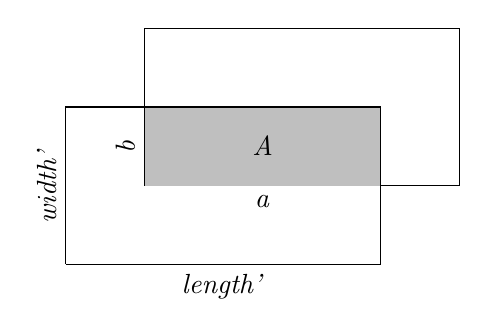
\begin{tikzpicture}
    \draw (0, 0) -- (0,2) -- (4,2) -- (4,0) -- (0,0);
    \draw (1,1) -- (1,3) -- (5,3) -- (5,1) -- (1,1); 
    \draw [fill=lightgray] (1,1) -- (1,2) -- (4,2) -- (4,1);
    \node [below] at (2,0) {\textit{length'}};
    \node [above, rotate=90] at (0,1) {\textit{width'}};
    \node [below] at (2.5,1) {\textit{a}};
    \node [above, rotate=90] at (1,1.5) {\textit{b}};
    \node at (2.5,1.5) {\textit{A}};
\end{tikzpicture}    